\chapter{Tight Binding Recursion}
\section{The Local Atomic Environment}
  Vol.~35 of Solid State Physics is dedicated to electronic structure
theory from the point of view of the local environment. This perspective
has a long tradition in physical and chemical electronic structure theory.

  Topics that are often discussed at the beginning of introductory physics courses include:
the study of black body radiation, photoemission phenomenon, De Broghlie waves,
electron diffraction experiments and the structure of the hydrogen atom.
Examination of thesis topics constitute a suitable foundation 
for understanding the formalism and experimental justification for the theory.

  It is natural to hope that from the understanding of the electronic states of hydrogen the
understanding of larger atomic systems, containing progressively more electrons, might emerge. 
However as the number of electrons in a system grows the wave function becomes 
somewhat unwieldly to work with and the accurate evaluation of the 
electron-electron repulsions becomes more difficult. Computers provide a route
to numerical solutions of the equations governing the behaviour of these systems.

Computer simulations are commonly performed these days in many branches of physics, 
chemistry, engineering, and biology. The use of computers to solve Schr\"odinger's 
equation for electrons in crystals has led to the proliferation of the 
many, many tribes of electronic structure theory. 

The tribes are well known to practitioners in the field. A non-exhaustive list
of some of these we can name here as: tight binding and linear combination of atomic orbitals (LCAO), 
linear muffing tin orbitals (LMTO), plane waves and pseudopotentials, Gaussian orbitals, and 
Kohn-Kuttinger-Rostiger theory.

While successful in a number of respects numerical work can be tedious and, more importantly, can obscure underlying
mechanisms. There is also a tendency for people working in numerical methods to become 
excessively obsessed with algorithmic details and, most importantly,
the results of a single calculation may not provide a framework that accounts for a range
of phenomenon in homologous series of materials where only slight adjustment of the physical
interaction parameters change. (This speaks to Ehrenreich third observation that results for homologous materials should be computed
wherever possible and the results should be compared). 

An example of the economy of explanatory expression afforded by the recursion method
and a physical formulation in terms of the local atomic environment
is Ref.~\cite{johannes76}. In that work 76 crystal structures are correctly predicted 
with a model containing 5 parameters, a determinedly naive numerical approach would
require computing the total energies of each of those structures and comparing them directly.

The purpose of this note is two fold: firstly to attempt to summarize the incredible range and
detail of theory and application covered in Vol. 35 of Solid State Physics; secondly, to speculate on where 
it should be possible to exploit modern computational advantages and new understanding 
which has emerged in materials to systematically improve descriptions of quantum systems based
on the local environment. 

\section{The Invariance Theorem}
\label{sec:invariance}
Heine presents an extended discussion of the invariance
theorem. Heine's section begins, by way of introduction, by pointing 
out an analogy between the the local density of states of a system of interacting
electrons and the black body spectrum of electromagnetic radiation.
Weyl [1911 Math. Ann. 71 441] demonstrated demonstrated the total density
of modes is independent of the shape of the cavity so long as the
radiation is contained in a cavity with dimensions greater than the wavelengths
under consideration. Von Laue [1914 Ann. Phys. Lpz 44 1197] demonstrated that the local density of modes at 
a particular point are exponentially insensitive to the cavity walls.

This analogy has been developed by Friedel [1954 Adv. Phys. 3 446] where
the substition is electromagnetic modes for electronic wavefunctions and
the probability density for finding an electron at a given point
with a given energy replaces the local density of normal modes.\cite{annett94}

The analogy can be seen by writing the density of states,
and the local density of states (for each spin direction) as:
%
\begin{eqnarray}
n(E) = \sum_{n}\delta(E-E_{n}) \\
n(E,\r) = \sum_{n} |\psi_{n}(\r)|^{2}\delta(E-E_{n})
\end{eqnarray}
%

The local density modes of black-body radiation alternatively can be written:
%
\begin{equation}
\rho(\omega,\r)= \sum_{i} |\bra \r| \psi_{i}\ket|^{2}\delta(\omega-\omega_{i}),
\end{equation}
%
with $\psi_{i}$ the eigenfunction (of an electromagnetic wave or a wavefunction) for an eigenvalue $\omega_{i}$.\cite{annett94}
The normal modes of a system can be quite quite sensitive to disturbances but the 
local density of modes, averaged over a small frequency interval, is a stable quantity 
insensitive to disturbances more than a few wavelengths away.

The local density of states is related in turn to the Green's function of a system:
%
\begin{equation}
n(E,\r) = -\frac{1}{\pi}{\rm Im}~G(\r,\r',E)
\end{equation}
%

\section{Matching Green's Functions}
First a change of variables is perform from $\r$ to $\r''$ in 4.1 and $\r$ to $\r''$ and $\r'$
to $\r$ in 4.3:
%
\begin{equation}
\label{eq:greentot}
[-\frac{1}{2}\nabla^{2}_{\r''} + V(\r'') - E]G(\r'',\r',E)= -\delta(\r''-\r')
\end{equation}
%
\begin{equation}
\label{eq:greenA}
[-\frac{1}{2}\nabla^{2}_{\r''} + V(\r'') - E]G_{A}(\r,\r'',E)= -\delta(\r''-\r')
\end{equation}

Now multiply Eq.~\ref{eq:greentot} by $G_{A}$ and Eq.
\ref{eq:greenA} by $G$ Then integrate over $\r''$ over region A using
Green's theorem:
%
\begin{equation}
\label{eq:greenthm}
\int\int\int(\phi\nabla^{2}\psi - \psi\nabla^{2}\phi)d^{3}\r 
= \int(\phi\nabla\psi-\psi\nabla\phi)d{\mathbf{S}}
\end{equation}
%
We suppress the energy arguments from here on in assuming them to be contained in G. 

obtained by expressions for $G$ by integrating $\r''$ over region $A$.
%
\begin{equation}
\label{eq:green1a}
G(\r,\r') = G_{A}(\r,\r') + \frac{1}{2} \int d\mathbf{S} 
[\frac{\partial G_{A}(\r,\r_{s})}{\partial n_{S}}G(\r_{S},\r') - G_{A}(\r,\r_{S})\frac{\partial G(\r_{S},\r')}{\partial n_{S}}] [\r, \r' \in A]
\end{equation}

$\frac{\partial}{\partial n_{S}}$ denotes the normal component of grad across
the surface S and $\r_{S}$ is a point on S. (The grad term is a directional component
so the sign can change depending on the orientation.)

And in region B:
%
\begin{equation}
\label{eq:green1b}
G(\r,\r') = G_{B}(\r,\r') - \frac{1}{2} \int d\mathbf{S} 
[\frac{\partial G_{B}(\r,\r_{s})}{\partial n_{S}}G(\r_{S},\r')
- G_{B}(\r,\r_{S})\frac{\partial G(\r_{S},\r')}{\partial n_{S}}] [\r, \r' \in B]
\end{equation}
%

A further property has been used:
%
\begin{equation}
G(\r,\r',E) = G(\r',\r,E),
\end{equation}
%
which is often justified on the ground of a time reversal theorem applying 
to the wave functions in the system.

Finally consideration of the case where $\r'$ and $\r''$ are in different regions is required.

With $\r''$ in B and $\r'$ in A Eq.~\ref{eq:greentot} becomes:
%
\begin{equation}
[-\frac{1}{2}\nabla^{2}_{\r''} + V(\r'') - E]G(\r'',\r') = 0,
\end{equation}
%
the delta function is uniformally zero with those spatial constraints.

The next case restricts $\r$ in B:
%
\begin{equation}
[-\frac{1}{2}\nabla^{2}_{\r''} + V(\r'') - E]G_B(\r,\r'')= \delta(\r-\r''),
\end{equation}
%

A similar cross multiplying trick gives:
%
\begin{equation}
\label{eq:green1c}
G(\r,\r') = -\frac{1}{2} \int dS[\frac{\partial G_{B}(\r, \r_{S}}{\partial n_{S}} G(\r_{S},\r')
- G_{B}(\r, \r_{S})\frac{\partial G(\r_{S},\r')}{\partial n_{S}}] \quad [\r~{\rm in}~B, \r'~{\rm in}~A],
\end{equation}
%
and a similar relation for [$\r$ in A and $\r'$ in B].

Eq.~\ref{green1a} and Eq.~\ref{green1b} give solutions for G but 
aren't very useful until the terms $G(\r_S,\r)$ and 
$\frac{\partial G}{\partial n_{S}}$ are eliminated.

From Eq.~\ref{eq:green1a} we let $\r$ tend to the boundary so $\r = \r_{S}$
%
\begin{equation}
\label{eq:greensys1}
G(\r'',\r') = G_{A}(\r''_{S}, \r') + \frac{1}{2} \int d{S}
[\frac{\partial G_{A}(\r''_{S}, \r_{S})}{\partial n_{S}} G(\r_{S},\r) - 
G_{A}(\r''_{S},\r_{S})\frac{\partial{G(\r_{S}, \r')}}{\partial n_{S}}].
\end{equation}
%

The second relation comes from Eq.\ref{eq:green1c} with 
$\r$ in region B and letting $\r$ tend to $\r^{''}_{S}$.
%
\begin{equation}
\label{eq:greensys2}
G(r''_{S}, \r') = -\frac{1}{2}\int dS [\frac{\partial G_{B}(\r''_{S}, \r_{S})}{\partial n_{S}}
-G_{B}(\r''_{S},\r_{S})\frac{\partial G(\r_{S},\r')}{\partial n_{S}}]
\end{equation}
%

We now dump the cumbersome indices on the position attributes. These
were necessary to motivate the physical argument for how we have a Green's function
description in one region of space, a Green's function description in another, 
and the joined physical system should be some combination of these two descriptions
which match at the interface. The final step is to write Eq.~\ref{eq:greensys1} 
and Eq.~\ref{eq:greensys2} as matrices:
%
\begin{eqnarray}
\label{eq:operator1}
\g = \g_{A} + \frac{1}{2}\G'_{A}\g - \frac{1}{2}\G_{A}\g' \\
\g = -\frac{1}{2}\G'_{B}\g + \frac{1}{2}\G_{B}\g' \\
\end{eqnarray}
%
\begin{eqnarray}
\label{eq:operator2}
\g & = & [\G^{-1}_{A}(1-\frac{1}{2}\G'_{A}) + \G^{-1}_{B}(1+\frac{1}{2}\G'_{B})]^{-1} \G^{-1}_{A}\g_{A} \\
\g' & = & [(1-\frac{1}{2}\G'_{A})^{-1}\G_{A} + (1+\frac{1}{2}\G'_{B})^{-1}]^{-1}(1 - \frac{1}{2}\G'_{A})^{-1}2\g_{A}
\end{eqnarray}
%
$\g$, $\g_{A}$, $\g'$ are vectors in a space $\{\r_{S}\}$ with components $G(\r_{S},\r')$,
$G_{A}(\r_{S},\r')$, $\partial G(\r_{S},\r')/\partial n_{S}$ with $\r'$ fixed and
$\G_{A}$, $\G'_{A}$ are operators in the space with matrix elements
$G_(A)(\r''_{S}, \r_{S})$, $\partial G_{A}(\r''_{S}, \r_{S})/\partial n_{S}$.

Where the inverse in Eq.~\ref{eq:operator1, eq:operator2} 
doesn't exist there is a pole. This is the condition for a discrete energy level 
of the Schrodinger equation for the combined A + B systems. 

Equations written in the form of \ref{eq:green1a} are of the type required for the invariance theorem namely:
%
\begin{equation}
G(\r,\r';E) = G_{A}(\r,\r';E) + {\rm boundary ~ corrections},
\end{equation}
%
where we have restored the energy argument.
These considerations provide a reasonable mathematical framework for 
investigating electronic structure from the point of view of the local environment.
Indeed as Heine himself says: 

\begin{quote}
The importance of this approach would lie in the fact that
one has a single entity $G_{A}$ to represent an element in anything 
from a small molecule to a complex alloy.
\end{quote}

As a practical example the success of planewave and pseudopotential methods 
is reliant on finding decent approximations to the quantity $G_{A}$. The plane waves
in the interstitial regions must match the Green's function for the atomic system
at a particular radial cutoff energy and eigenvalue. If a function can be found that 
describes the scattering of these waves across a suitable energy range the approximation 
is a good one and the matching of the two systems will be successful.

Heine's ambition turns on this:
%
\begin{quote}
We see now that the trick in the new formulation of quantum 
mechanics is not just to express measurable quantities in terms of 
G, {\emph but in terms of some appropriate small parts of G that can be solved 
for and computed separately from all the unwanted remainder of G.}
\end{quote}
%
This relies, again in analogy with black bodies, on the Green's
function in a certain region of space being independent of the size and shape
of the container and the boundary conditions.

\section{Recursion Method}
  The principle of the recursion method is to obtain a convergent expression 
for an element of the Green's function:
%
\begin{equation}
G_{\chi\chi}(E) = \bra\chi|[E + i\delta -H]^{-1}|\chi\ket.
\end{equation}
%

The Green's function can be immediately related to the local density of states as:
%
\begin{equation}
n_{\alpha l}(E) = -\frac{1}{\pi} {\rm Im}\bra\alpha l|[E + i\delta -H]^{-1}|\alpha l\ket
\end{equation}
%

The state $\chi$ which we project on to can be made up of some linear combination 
of the local basis set $\phi_{\alpha l}$, which, in turn, could be local atom centered orbitals, bond orbitals, 
Wannier functions, atomic diplacements, or any localized quantity we wish to define. The method is thus
applicable to a wide range of problems in condensed matter. In short what we wish to examine
is determined by the choice of $\chi$.

\subsection{Mathematical Origin}
The trick of the recursion method, if you like to think of things in terms of tricks, 
or its generating feature, if you prefer, is that from the outset the `Greenian', the element
of the Green's function we are interested in, is restricted to a particular matrix element: 
%
\begin{equation}
\label{eq:greenian}
G_{00}(E) = \bra u_{0}|[E-H]^{-1}|u_{0}\ket 
\end{equation}
%
As Heine puts it in his chapter:
%
\begin{quote}
Note that we do not want the whole of the inverse matrix $[E-H]^{-1}$, 
\emph{only one element}, and on this the whole method depends. In physics we do not
usually inquire about the whole of life, but about one particular matrix element (at a time) and we have chosen
$u_{0}$ so that Eq.~\ref{eq:greenian} gives us what, to put it crudely, we want.
\end{quote}

Eq.~\ref{eq:greenian} can be rewritten in terms of its determinants:
%
\begin{equation}
\label{eq:greendet}
\bra u_{0}|[E-H]^{-1}|u_{0}\ket = \frac{{\rm det}|D_{1}|}{{\rm det}|D_{0}|},
\end{equation}
%
or, equivalently, be written as:
%
\begin{equation}
\label{eq:greendet}
\bra u_{0}|[E-H]^{-1}|u_{0}\ket = \frac{1}{\frac{{\rm det}|D_{0}|}{{\rm det}|D_{1}|}}.
\end{equation}
%
Appeal is then made to Cauchy\footnote{Baron Augustin-Louis Cauchy FRS FRSE (21 August 1789 – 23 May 1857)} 
for the following expansion:
%
\begin{equation}
{\rm det}|D_{0}| = (E-a_{0}){\rm det}|D_{1}| - b^{2}_{1}{\rm det}|D_{2}|
\end{equation}
%
and when generalized to determinants for $|D_{n}|$, $|D_{n+1}|$, and $|D_{n+2}|$:
%
\begin{equation}
\frac{{\rm det}|D_{n}|}{{\rm det}|D_{n+1}|} = E -a_{n} - \frac{b^{2}_{n+1}}{\frac{{\rm det}|D_{n+1}|}{{\rm det}|D_n+2|}}
\end{equation}

The chain model has been used in numerical work as a way of diagonalizing matrices in a computer 
C. Lanczos J. Res. Natl. Bur. Stand. 45, 255 (1950) and
by Chebyshev for approximating functions on an interval
P. L. Chebyshev, Bull. Acad. Imp. Sci. St. Petersbourg 1, 193 (1859)

%\begin{equation}
%b_{n+1}|u_{n+1}\ket = H |u_{n}\ket - a_{n}|u_{n}\ket - b_{n}|u_{n-1}\ket
%\end{equation}

\section{Integrals of the Density of States}
%
Some integrated quantities over the density of states of interest.

The electron occupancy of a specific orbital:
%
\begin{equation}
N_{\alpha l}(E) = \int_{-\infty}^{E_{F}} n_{\alpha l}(E') dE'
\end{equation}
%

The total energy in a particular orbital:
%
\begin{equation}
U_{d} = \int_{-\infty}^{E_{F}}E'n_{\alpha l}(E') dE'
\end{equation}
%

The energy difference of two structures A and B can also be computed
to high accuracy:
%
\begin{eqnarray}
\label{eq:Ua}
U_{A} = \int_{-\infty}^{E_{FA}} E n_{A}(E) dE
\end{eqnarray}
%
\begin{eqnarray}
\label{eq:Ub}
U_{B} = \int_{-\infty}^{E_{FB}} E n_{B}(E) dE
\end{eqnarray}
%
\begin{equation}
\label{eq:totaldos}
Z = \int_{-\infty}^{E_{FA}} n_{A}(E)dE = \int_{-\infty}^{E_{FB}}n_{B}(E)dE
\end{equation}
%
\begin{equation}
U_{A}-ZE_{FA}= \int_{-\infty}^{E_{FA}}(E-E_{FA})n_{A}(E)dE
\end{equation}
%
\begin{equation}
U_{B}-ZE_{FA}= \int_{-\infty}^{E_{FA}}(E-E_{FA})n_{B}(E)dE + \int_{E_{FB}}^{E_{FA}}n_{B}(E)dE
\end{equation}
%
If $n_{B}(E)$ is taken to be constant across that small energy range, the second term, in
Eq. results in a small squared term that can be dropped. Swapping $E_{FB}$ and $E_{FA}$ gives
a similar result. This justifies dropping the A index on the Fermi energy to get the
final expression:
%
\begin{equation}
U_{A}-U_{B} = \int_{-\infty}^{E_{F}}(E-E_{F})[n_{A}(E) -n_{B}(E)]dE.
\end{equation}
%
It is this expression used to separate the Lave phases of transition metals in Ref.~\cite{haydock76}.

\section{Practical Recursion}
An example from Kelly helps to make the application of the scheme clear:
%
\begin{quote}
As input data we require a convenient local representation of $H$. In simple crystals,
this is most easily given in terms of interactions with a unit cell and between neighboring cells.
For a fcc transition metal we have nine orbital (1 s-orbital, 3 p-orbitals, 5 d-orbitals) per site, and a diagonal 9x9 matrix
for the self-energies of these orbitals. Twelve 9x9 matrices suffice to describe the interaction 
of any atom with its nearest neighbors.
\end{quote}
%

The actual operations of $H|u_{n}\ket$ which have been discussed, in a general way so far, 
can be written as:
%
\begin{equation}
H|u_{n}\ket = \sum_{\alpha l \beta j}a_{n \alpha l}(\bra \beta j |H| \alpha l\ket)|\beta j\ket,
\end{equation}
%
to exploit the sparsity of H we introduce an index $z$ which runs over the neighbors of 
site l with which the orbitals interact:
\begin{equation}
H|u_{n}\ket = \sum_{\alpha l z}a_{n \alpha l}(\bra \beta_{z} j_{z} |H^{z}|\alpha l\ket)|\beta_{z} j_{z}\ket.
\end{equation}

There are no restrictions on the number of orbitals per site, or on the range of interactions that can be
incorporated, these only impact on the efficiency of the method and the validity of the original assumptions
about the dominance of the local atomic environment.

\section{Future Work}
The references in Vol. 35 demonstrate the scope of application of the method 
already achieved by 1980. A subset of those works have been referenced here. 
Haydock's conclusion is interesting in he gives prognosis for further work
along two lines. 

The first line of research consists of diffusing quantum processes in disordered
solids:
%
\begin{quote}
One of the outstanding problems is that of the Anderson model
of a disordered solid. Here the Hamiltonian is defined statistically and
one would like to transform to a corresponding statistically defined chain where
one could discuss the distributions of various physical quantities.
\end{quote}
%

The second line of inquiry consists of the extension of the recursion from a single 
particle description of electronic structure to a many-body Hamiltonian.
%
\begin{quote}
Finally, the reader may have noticed that the approach of this chapter has been entirely directed
toward independent particle models. However, many-body Hamiltonians must be similarly 
transformable to chain models. Aside from a small amount of thought and continuing interest, 
nothing has been done about this and it remains a most interesting problem concerning recursive 
solution of the Schrodinger equation.
\end{quote}

In fact work did continue in this field. In Ref.~\cite{annett94} the local density of states (LDOS)
is extended to the projected density of transitions (PDOT) and it is argued singularities
in the PDOT correspond to thresholds for creating long lived elementary excitations 
of the many body system.

In the rest of this note we will consider the possibile extensions of the recursion method.
For the first we will consider the possibility of treating the diffusion of hydrogen 
in a lattice with varying degrees of disorder. In the second we will consider the extension
of the recursion method to performing GW type calculations.


\section{Many Body Recursion}
\label{sec:manybodyrecursion}
	Since Vol. 35 was published there has been a rise in the accessibility of density functional methods 
and the access to good single particle approximations to the electronic eigenstates of a crystal
is routine. Additionally progress on the problem of determining unique approximations to localized
electronic states, Wannier functions, means tight binding Hamiltonians can be parameterized directly
rather than via fits to band structures and relying on physical intuition. Finally ab initio many body
calculations have also proved quite successful

A many body Hamiltonian amenable to being written in a sparse format might look like this:
%
\begin{equation}
H = [\frac{1}{2}\nabla^{2} + \tilde{v}_{\rm loc} + \hat{\Sigma}(\r,\r';\omega)]
\end{equation}
%
	$\Sigma(\r,\r';\omega)$ is a self energy operator, it is not local and 
has an additional argument that includes the energy.
If we impose a requirement that spatial integrals over $\Sigma$ are performed in 
well defined atom centered regions of space with localized Wannier functions. 
The off diagonal elements of a tight binding Hamiltonian can be quantified as:
%
\begin{equation}
\int_{\Omega_{j}}\bra w_{i}(r-R)|\Sigma(\R,\r';\omega)|w_{j}(r-R)\ket d\r'
\end{equation}
%
	Subsequent neighbour interactions would take a similar form
with the integration region, $\Omega_{j}$ being a Wigner cell around an 
atom with its Wannier center at $\R_j$. In order for the scheme to be sensible the contributions from subsequent shells 
must be negligible. This is likely to be the case so long as either the atomic orbitals $w$ and/or $\Sigma$ 
fall off quickly enough. Which, as will become clear when we discuss
the relationship of this scheme to the GW approximation, requires 
the Green's function or the screened Coulomb interaction to be sufficiently localized.

The on-site self-interaction term can be computed as
%
\begin{equation}
\int_{\Omega_{i}}\bra w_{i}(\r-\R_{i})|\sigma(\r,\r';\omega)|w_{i}(\r-\R_{i})\ket d\r'd\r
\end{equation}
%
The self-consistency in the recursion method relies on the adjustment of the $\Sigma$ operator 
and the fewer depths of recursion required to stabilize this quantity the more efficient the
scheme can be considered.

In principle we can now compute any quantity we like that can be expressed
as a density of states, or an integral over the density of states.
The basis set may remain an issue. The localized functions will not have the 
flexibility of planes waves so if we seek the green's function in the 
region of the plasmon energies our basis set might not have the flexibility 
to describe that solution? I'll have to think about this. Ultimately the 
solution for the resolvent at those energies i.e. ${\rm Im} G_{nk}(\omega)$ should 
reproduce what I'm looking for. The test for this would be with Si, if 
I can reproduce spectral functions with TB recursion that is a legitimate 
proof of concept and would clarify the extent to which collective excitations,
plasmon, can be incorporated in TB recursion. 

Also Writing the equations in this way and the proposed method of solution
yield some post hoc justification for parameterizations of plasmon
pole models or the use of Pad\'e approximants to capture the frequency dependence
of the key operators.

Similarly the contributions of neighbours to the self-energy 
operator yields some physical insight.

\section{The Self-Energy From Multiple Greenian Elements}
  A good first order approximation to $\Sigma$ comes from the GW approximation.
We will write matrix elements of this to see the connection between the
recursion method and the calculation of $\Sigma$. It should be come apparent that computing
the self-energy requires a large table of Greenian matrix elements between states localized
on nearby atoms, far away atoms, and the entire valence and conduction band spectrums. 
This table of Greenian elements could become excessively large very quickly and requires some
rigorous procedure to map it back into a manageable scale.
%
\begin{equation}
\label{eq:sigma}
\Sigma_{ij}(\omega) = \bra\phi_{i}|\int G(\omega-\omega')W(\omega')d\omega'|\phi_{j}\ket
\end{equation}
%
	We now insert the identity operator into Eq.$\sigma$ strategically and at 
a number of places:
%
\begin{equation}
\label{eq:sigma}
\Sigma_{ij}(\omega) = \bra\phi_{i}|\int G(\omega')\sum_{n}|\phi_{n}\ket\bra\phi_{n}|(G(\omega')|\phi_{n}\ket\bra\phi_{n}|G(-\omega')v)d\omega'|\phi_{j}\ket
\end{equation}
%
\begin{equation}
\label{eq:sigma_onsite}%need to check the frequency polarization expression
\Sigma_{ii}(\omega) = \bra\phi_{i}|\int G(\omega')\sum_{n}|\phi_{n}\ket\bra\phi_{n}|(G(\omega')|\phi_{n}\ket\bra\phi_{n}|G(-\omega')v)d\omega'|\phi_{i}\ket
\end{equation}
%
The insertion of multiple identity operators makes what we need clear. What is required 
is to tabulate the Greenian's, $G_{ij}(\omega)$, between eigenstates of the system
the non-interacting system. In {\it ab initio} calculations this requirement 
gives rise to the "sum over states" problem. Although in principle the valence
and conduction states, at every wave vector, are known their calculation and storage
is tedious, and justified truncation of the sum is problematic.

For this scheme to be workable we again stress that the system interaction
must be sufficiently local such that $Sigma_{ij}$ matrix elements can be
calculated. This corresponds to the mutual interaction of the electrons being 
short ranged. For a single particle tight binding model these off diagonal hopping
elements can be calculated and are fixed. It is this interaction we wish
to generalize slightly to allow for a component of dynamical interaction.

\section{The Project Density of Transitions}
  The PDOT\cite{annett93, haydock00, haydock16} method is 
appropriate for calculating the polarizability and provides a direct physical
interpretation in a many electron system. 

Written in Hedin's scheme the polarizability 
takes the form of a term: $iGG$, in Feynman diagrams this is a bubble diagram. We need to calculate the propagator
of an electron from 1 to 2, and a hole from 2 to 1. Dimensionally, after a Fourier transform,
the polarizability has units of transition probability per unit energy. Where there are discrete
states there are discrete transitions, this would be the case for systems
that could be considered molecules, where there are continuous bands there are continuous
bands of transitions, in metallic crystals this would be the case.

Where the recursion method for the PDOS computes the final energy distribution
for a stationary state in the syste

\begin{figure}
\includegraphics{./invariance/schematicpolestructure.pdf}
\end{figure}

I think Umari's operator for $|\phi\ket\bra\phi|$ would be a natural way of
approximating the necessary sums that are complimentary to the chosen
localized single particle states (both valence and low lying conduction).
We then have the continuum states as $|\phi\ket=e^{i\G\cdot\r}-<\G|w_{i}(\r-\R)>$,
with the occupied and low lying conduction manifold represented as Wannier 
functions and the $|\phi>$ states as orthogonalized plane waves.

	Although this is essentially just a rewriting of Hedin's equations
it has practical consequences. The present method eliminates
burdensome storage of what are in practice gigantic Green's function, 
screened Coulomb, and self-energy matrices. It also 
stabilizes the necessary numerical integrations and convolutions in frequency space. 
The quadrature methods used in the standard recursion theory remain applicable.

These savings are obtained at the price of a nested call stack of recursions which 
in principle must be infinite. This may seem troubling but we do intend to truncate
the level of recursion at some point and the depth of the recursive call stack should
equate to the number of terms in the self energy expansion that are required.

	Careful, justified, selection of the initial wave functions and tight binding parameters
is also required and these quantities (if they are not chosen to be analytic and approximate)
must be computed and stored. However work done on Wannier functions makes this a very
practical route. We will now embark on some numerical work in the hope that satisfactory 
results can be obtained by truncation of the recursive call stack at a manageable level. 

Finally the method requires computation of the initial stationary states of the system.

The electron addition operator:
%
\begin{equation}
[H, c^{\dagger}(t)] = -i\hbar \frac{d}{dt} c^{\dagger}(t).
\end{equation}
%
The operator will evolve into a superposition of a fraction of the 
possible transitions of the system. If a complete set of orthonormal $\{P_{\zeta}\}$ 
states is introduced the projected transitions can be written:
%
\begin{equation}
\psi_{\alpha} = \sum_{\zeta\eta} P_{\zeta}c^{\dagger}P_{\eta} \qquad \epsilon_{\alpha} = E_{\zeta} - E_{\eta}
\end{equation}
%
The PDOT is then:
%
\begin{equation}
\label{eq:ehpairs}
\mu(\epsilon) = \sum_{\alpha} \bra\psi_{\alpha}^{\dagger}|\psi_{\alpha}\ket \delta(\epsilon-\epsilon_{\alpha})
\end{equation}
%
The stationary states all have infinite lifetimes, and according to Haydock, \ref{eq:ehpairs} can
be interpreted as the probability distribution in energy for the decay of a bare electron into one dressed
with electron-hole pairs.

It is possible to formulate this in terms of discrete transitions for low energies, for high energies
the initial state is clearly going to diffuse outwards very far and result in the excitation of 
many oscillators throughout the crystal. Where the complete set of orthonormal states
hasn't been computed already (this refers to the sum over states problem) it is required to directly
calculate the PDOT. Haydock gives a prescription for this the time dependent behaviour of
an operator is given:
%
\begin{equation}
\label{eq:creationt}
c^{\dagger})t_ = exp{i\mathbf{L}t/\hbar} c^{\dagger}
\end{equation}
%

The super-operator $\mathbf{L}$ is defined on a operator $\mathbf{x}$
%
\begin{equation}
\mathbf{L} \mathbf{x} = [\mathbf{H}, \mathbf{x}]
\end{equation}
%
Eq.~\ref{eq:creationt} will only converge if the interactions are expanded in termed
of the screened interaction. The mechanics discussed in the the project density of 
transitions is equivalent to the Hedin's GW approximation, and provides a framework
for computing the renormalization in terms of local orbitals and an 
effective energy band correponding to the plasmons.

With the choices $u_{0}=c^{\dagger}/<c c^{dagger}>^{\frac{1}{2}}$, $u_{-1}=0$,
subsequent operators are:
%
\begin{equation}
\label{eq:pdotvectors}
\mathbf{u}_{n+1} = (\mathbf{L} \mathbf{u}_{n} - a_{n}-b_{n}\mathbf{u}_{n-1})/b_{n+1}
\end{equation}
%
\begin{equation}
a_{n} = \bra u^{\dagger}_{n} \mathbf{L} \mathbf{u}_{n} \ket
\end{equation}
%
\begin{equation}
b_{n+1} = \bra 
(\mathbf{L} \mathbf{u}_{n} - a_{n} \mathbf{u}_{n} - b_{n}u_{n-1})^{\dagger} 
(\mathbf{L} \mathbf{u}_{n} - a_{n} \mathbf{u}_{n} - b_{n}u_{n-1})
\ket^{\frac{1}{2}}
\end{equation}
%

This recursion rarely terminates in practice due to loss of orthogonality of
the vectors or because the subspace is too large to compute.

If the PDoT consists of a single band of transitions with a known width 
and energy,then the recurrence can be continued with constant matrix elements, $a_{n}$ and $b_{n}=b$
for $n>N$ where a and b are fit to the known band. 

For interacting bands it becomes more difficult to approximate a 
single effective energy band.

The termination of the recurrence is a very important point. 
We are interested in the excited state properties of a system (N+1, N-1) electrons
from a local perspective. In Chapter.~\ref{chap:invariance} we worked hard to collect work
justifying this perspective. A plasmon is the collective variable of the electronic system.
In a continued fraction expansion of the the PDoT more and more distance transitions are coupled
to the starting transition. In a real system the continued fraction will terminate at the surface,
however if the surface atom is changed by a small number of atomic positions it would
be very surprising if the collective plasmon modes of the cavity changed. 
Picking a value of anywhere from 30-60 moments away should help the reader to visualize this.
The contribution of successive transistion are finite, in reality there are not an infinite number
of hops, and the effect of these remote transitions can be mapped onto collective variables.

For silicon, the plasmon energy band occurs around 16 eV. This is very high compared
to the single particle excitations which occur around 1 eV. The long range $1/\r$ nature of the Coulomb
interaction means electrons are coupled over large distance.
This coupling accounts for the high excitation energy: to get the
electron cloud moving collectively requires a relatively large amount of energy.

Experience with the GW approximation indicates an effective band model works very well
for sp semiconductors \cite{godbyneeds, hybertsenlouie, bergstressen}. 
A single plasmon mode approximates the long range density of transitions, and the local
atomic environment contributions to the PDoT can then be captured directly with the standard nearest
neighbour hopping and the inclusion of the lowest energy single particle transitions.

The situation for transition metals will be more complicated but again the local approach should yield 
a tractable framework. The important low energy transitions can all be include as explicit single particle states
in the Hamiltonian (spin resolved states). The remaining particle-hole renormalization would then
be accounted for via a set of effective plasmon energy bands. It would be of interest to
see how the number and position of these effective bands can change between systems.

The projected transitions can be written:
%
\begin{equation}
\mathbf{\psi}_{\alpha} = \sum_{n} \psi_{n}(\epsilon_{\alpha})\mathbf{u}_{n}
\end{equation}
%
the sum is over the basis ${\mathbf{u}_{n}}$ generated by Eq.~\ref{eq:pdotvectors}
with coefficients generated by:

\begin{equation}
\label{eq:pdotcoeff}
\psi_{n+1}(\epsilon) = ((\epsilon-a_{n})\psi_{n}(\epsilon) - b_{n}\psi_{n-1}(\epsilon))/b_{n+1}
\end{equation}

In his paper Haydock says equation \ref{eq:pdotcoeff} has two linearly independent solutions
which can be combined to satisfy the boundary conditions on $\psi_{N+1}$ or $\psi_{-1}$ or both.
Physically I understand this as choosing where the recurrence begins and ends not completely
clear on what it implies mathematically.

The $\mathbf{u}_{0}-\mathbf{u}_{0}$ element of the resolvent is
%
\begin{eqnarray}
R(\epsilon)& = & 1/\epsilon-a_{0}-b_{1}\psi_{1}(\epsilon)/\psi_{0}(\epsilon) \\
  & = & 1/\epsilon-a_{0}-b^{2}_{1}\epsilon-a_{1}-b^{2}_{2}\epsilon ... b_{n^{2}}/epsilon-a_{n}
\end{eqnarray}
%
and finally the PDoT:
%
\begin{equation}
\mu(\epsilon) = -\bra \mathbf{c} \mathbf{c}^{\dagger}\ket {\rm Sing} \frac{R(\epsilon)}{2\pi i}
\end{equation}
%
The PDoT is the residue of the resolvent which contributes to integrals enclosing the 
real $\epsilon$-line and it is normalized to the projecting operator.

Calculating how much of the sum rule is exhausted will give a good indication
of the effectiveness of a single band approximation, or what is equivalent,
the truncation of the recursion at a suitable number of moments.

Finally a note from the perspective of plane waves and pseudopotentials. For
highly excited conduction band states. The Bloch periodic wave function is
essentially a plane wave or free electron state. This is equivalent to saying for
sufficiently high energy states the kinetic energy is the dominant term in the Hamiltonian.
For these plane wave states the Wannier transformation is a psinc function. These psincs
give a local representation of high energy plasmon modes.

\section{Appeal of A Local Formulation of Many Body Quantum Systems}
 A resonance or transition in k-space corresponds to an excitation 
of a crystalline eigenstate but the physical meaning of this is hard to access. Highly
localized states in $\k$-space correspond to relatively diffuse regions in real space. Where
transitions are formulated in terms of the local atomic environment the process becomes slightly
more intuitive. An electron creation operator $u_{0}$ generates the 
first excited state with eigenvalue $a_{0}$ in a particular unit cell. 
or viewed another way the creation operator takes the system to the energy 
of the $E_{N\pm1}$ interacting system depending on whether an electron or hole
was created. Eq.~\ref{eq:pdotvectors} will contain the contributions of the localized
wave packets in a vector $u_{\alpha}$ that corresponds to the resonance 
$\epsilon_{alpha}$. In an inverse photoemission experiment the $u_{alpha}$ chain
will come from the commutator of an electron creation operator, for a photoemission
experiment the chain of vectors in the excitation will correspond to creating a hole
in the electron system. An electronic wave packet interacts with its neighbours becoming
"dressed" by the nearby excitations of electron hole pairs. 

In a photoemission experiment real electric currents will be moving through the crystal as well.
Only the $\k$-component of the localized wave packet, at a given energy, will move through the crystal as 
an approximate eigenstate and can pass through without scattering so much that it can't be detected.
Furthermore the idea that there is a particular electron that gets excited and passes through the crystal
can't really be sustained. The initial wave packet is composed of all the electrons in the system, and its
propagation can't be assigned either. When the wave packet reaches the surface it can continue propagating
or be scattered back into the crystal, if it is to continue propagating the appropriate matrix element
is between the plane wave of the appropriate wave vector and the localized wave packet along with some
surface potential.

In this case we wish to study Greenian's between localized states and plane wave states.

Other processes mean the excited state can hop 
to its nearest neighbour leaving behind a hole. The recursive formula means
the coefficients of the continued fraction and the vectors are generated at
each step and the energy dependence of the interaction can be calculated 
in a close form. The trade off is the recursion depth must be sufficient to
pick up all the relecant poles of the interaction. For collective modes
the recursion depth would have to proceed to an impracticable depth which
is why we must map these contributions onto effective energy bands, collective
variables, or plasmon modes (depending on how you prefer to call them). The technique
clearly demonstrate the mathematical and physical justification of the plasmon as
collective excitations or a truncated series.

(The hole state and the excited state will also interact according to a coulomb interaction,
these are excitons, the radius of their (potentially) bound state being determined 
by the strength of the screened coulomb interaction and the shapes of the electron and hole
wave function. However the PDoT we are considering at the moment is just a 
single electron creation operator.
To calculate the PDoT for the electron hole system would require a 
two particle Green's function operator with a new pole in the spectrum forming
at the energy of the electron hole bound state.)

\section{Mori Memory Function}
\label{sec:morimemory}
  As noted in Ref.~\cite{annett94} there is a close connection between the PDOT
formalism and Mori's memory function. 

Interestingly when working on the diffusion
of hydrogen in a lattice I realised I would require a way of computing the
inverse Laplace transform of the continued fraction generated 
using Haydock's method. A quick search later and one of the first items to come up
was a paper titled "A Continued-Fraction Representation of the Time-Correlation
Functions" the first line of the abstract was, "A continued-fraction expansion of the Laplace
transform of the time-correlation functions is obtained...". It is very nice when a problem
arises where all you have to do is go to the shop and grab the solution off the shelf.

Like many store bought items some element of self-assembly is required. In this
section we wish to simplify Mori's analysis as much as possible so that we can directly 
apply the mathematical machinery of translating a continued fraction representation of
a diffusion problem into the time domain and extract measurable quantities.

The inner product, or matrix elements required to generate the coefficients 
$a_{n}$ and $b_{n}$ in Mori's approach are generalized to include a thermal averaging:

%\begin{equation}
%\label{eq:moriinner}
%(F, G^{*})= \frac{1}{\beta} \int_{0}^{\beta} \bra e^{\lambda H)Fe^{-\lambda H}G^{*}\ket d\lambda
%\end{equation}

There is a further computational advantage here. Though the inner product in Eq.\ref{eq:moriinner}
looks complicated, in fact, it only has the effect of altering the coefficients entering
the hopping matrix. This means the laplace transform computed from the continued fraction,
and the quantum mechanical hopping parameters can be computed separately.

Mori's formula allows us to interpret the spectral function in two ways. The first is as
a purely phenomenological one of an electron in a material being excited and as it passes through
a crystal on the way to a detector being scattered by the characteristic scattering modes of the
system. The electron from its initial bound state can interact with the many body system via
the plasmon modes available to it.

The second is to interpret the probe as measuring a statistical distribution of the 
renormalized many-body electron states which have spectral weight across the full
interacting energy spectrum. 

The former, via the Mori picture, is similar to the treatment of a free particle path
being modified by its interaction with atoms in what is termed Brownian motion. In the
case of a fermion in a crystal we are looking at its `brownian motion' as it interacts
with bosons on its way to a detector.

\section{Bullet Tight Binding Method}
\label{sec:bullet}
Bullet discusses some of the problems with treating d electrons in a tight binding 
formalism (Sec. IV 13 Solid State Physics Vol. 35). Fig. \ref{fig:datoms} demonstrates
one of the main issues arising with d electrons:
%
\begin{figure}
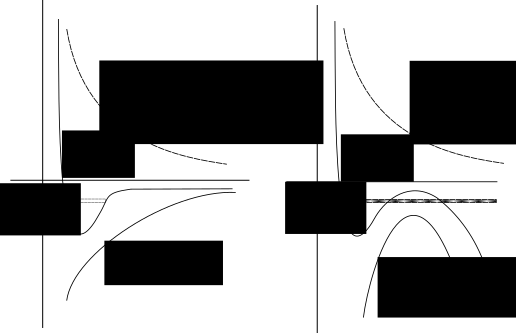
\includegraphics{./invariance/resonant-datoms.pdf}
\caption{The possibility of free electron states resonating with localized states.
The centrifugal components of the atomic d wave scattering channel can combine with
the atomic potential to produce a bound electronic state at some energy $E^{0}_{l}$ for an atomic system.
In a crystal the atomic periodic potential can be such that electrons can be bound in an
atomic d-like state can have the same energy as tunnel through the barrier localizing them and mix with free electron 
plane wave states. This dual character of the wave function, with localized components and extended components, requires careful 
detangling to return to a tight binding description. This difficulty stems from the presence of an energy resonance 
complicating the process of choosing the coefficients of the tight binding matrix. For the optimal, energy independent,
set of coefficients that can be chosen see the work of Pettifor. There is a close parallel with this resonant scattering of d-waves in materials
and Feschenbach resonances Ref.~\cite{chin10}.}
\end{figure}
%

From pseudopotentials we are familiar with having to match the logarithmic energy
derivative at some cutoff radius. Usually found by integrating the radial
Schr\"odinger equation to find $u_{l}(\r,\epsilon)$ and matching the logarithmic derivatives:
%
\begin{equation}
L_{l}(\epsilon) \equiv \frac{u'_{l}(\r_{0},\epsilon)}{u_{l}(r_{0},\epsilon)} = \frac{\kappa[j'_{l}
(\kappa r_{0}) - tan \eta_{l} n'_{l}(\kappa r_{0})]} {j_{l}(\kappa r_{0}) - tan \eta_{l} n_{l}'(\kappa r_{0})]},
\end{equation}
%
where
\begin{equation}
\label{eq:phaseshift}
\tan \eta_{l} = \frac{\kappa j'_{l} - L_{l}j_{l}}{\kappa n'_{l} - L_{l}n_{l}}.
\end{equation}

In terms of the energy and width the l=2 phase shift Eq. \ref{eq:phaseshift} 
can be written:
%
\begin{equation}
\label{eq:dshift}
\tan \eta_{d} = \frac{\frac{1}{2}W(\epsilon)}{\epsilon_{d}-\epsilon}.
\end{equation}
%
In Ref. \cite{friedel73} he notes the rest time for an electron on an atomic d state 
can be estimated at around $\hbar/W_{d}\approx 10^{-14}$s. In that paper he also
compares the relative merits of `muffin tin' calculations and tight binding approximations
the first approach he describes as leading, "to fairly exact if cumbersome
computations, and has thus had the support of the `computers lobby'".

The strong centrifugal contribution to the
atomic scattering potential from higher angular moment channels means the effective potential
can create a bound atomic state. In a solid the energy of this bound state can match the 
energy of a free electron state in the interstitial region and there will
be resonant tunneling between the two states. This results in the hybridization of d states
and plane waves. 

This means an appropriate model Hamiltonian must account for the various states as
%
\begin{eqnarray}
\label{eq:d-hamiltonian}
H = d-d  & d-PW \\
    PW-D & PW-PW \\
\end{eqnarray}
%
where d-d and PW-PW are of the tight-binding and plane-wave 
pseudopotential form and hybridization occurring in the 
off diagonal elements. 

These difficulty have been addressed in a number of works 
see, for example, D.G. Pettifor, J. Phys. C 5 97 (1972).
J. Hubbard Proc. Phys. Soc. London 92 921 (1967),
J. Hubbard and N. D. Dalton, J. Phys. C 1 1637 (1968),
and J. Hubbard, ibid 2, 1222 (1969). The problem being to define an
energy independent Hamiltonian, amenable to tight binding for the d electrons.

The $dd\sigma$ terms behave roughly as \cite{pettifor71}:
%
\begin{equation}
\label{eq:pettifor}
dd\sigma \approx \frac{-5W\cos\kappa_{d}R}{\kappa_{d}R}
\end{equation}
%
If we write our basis functions in terms of localized orbitals
Eq.~\ref{eq:pettifor} suggests our Hamiltonian matrix will be 
populated by a huge number of off diagonal matrix elements which can't be neglected. If 
the energy is equal to $k^{2}$ constructive interference occurs and the energy summation
diverges with off diagonal matrix elements between all d states on remote atoms becoming
significant. This isn't entirely surprising. We are considering a periodic crystalline solid
and the eigenfunctions of this crystal are extended throughout. The off diagonal elements
in a coordinate space representation reflect the long range cohesion of the material. See
Chapter \ref{chap:yang} for further discussion of this point.

The `best' approximations to the explicit formulas for $dd\sigma$, $dd\pi$ and $dd\delta$ and the phase
shift $d_{0}'$ of the diagonal tight-binding elements is given in D. G. Pettifor J. Phys. C. 2, 1051 (1969).
Whether we are able to create a tight binding description of transition metals
depends on whether a decent, energy independent, approximation to the electronic structure in fcc/bcc metals
can be achieved with 9x9 matrices describing nearest neighbour interactions of the s, p and d states,
in the Slater-Koster form.\cite{salter54}

\section{Slater-Koster Tight Binding}
  In a crystal if we denote the translation operator $\hat{T}$
as the one which shifts a the coordinates of a vector by a crystal lattice vector 
$\R_{i}$ we require firstly that $[\hat{T},\hat{H}]=0$, i.e. that the 
translation operator commutes with the Hamiltonian. This also
has the consequence that the eigenvectors of the Hamiltonian
must be eigenvectors of the translation operator. Bloch's 
celebrated theorem suggests that the eigenvalues of the 
translation operator acting on the eigenvector of a crystal is $e^{i\k\cdot\R}$.
If a basis set of atomic orbitals $\phi_{n}(\r-\R_{i})$
is placed on each atom in the crystal an un-normalized Bloch sum can be 
written as $\sum_{\R_{i}} e^{i\k\cdot\R_{i}}\phi_{n}(\r-\R_{i})$. For
a given $\k$ there will be off diagonal elements between bloch sums
for different atomic orbitals.

  Interestingly Slater and Koster state that there are no off-diagonal
elements of the Hamiltonian, consisting of the kinetic energy and the periodic potential, 
between Bloch sums with different $\k$'s. This is considered again in Chapter~\ref{chap:odlro}
where off diagonal elements in the Hamiltonian between different $\k$ values are exactly what give
rise to persistent currents.

  The matrix elements between Bloch sums (where L\"owdin orbitals $\psi_{n}$
are used instead of LCAOs) gives:
%
\begin{equation}
\sum_{\R_{j}} e^{i\k\cdot(\R_{j}-\R_{i})}\times\int \psi^{*}_{n}(\r-\R_{i})H\psi_{m}(\r-\R_{j})dV
\end{equation}
%
The development of computers means the secular equations can be solved 
at arbitrary $\k$ points. \footnote{The paper explicitly anticipates that the integrals and Bloch 
sums could be performed with the help of computers: "The possibility is not excluded 
that eventually ways will be found to do this work by means of high-speed computers, but
it will certainly be quite out of the question without such help."} 

The Slater-Koster work does however demonstrate in an intuitive fashion how localized atomic
waves, with different phases, can interfere (constructively or deconstructively) in order
to allow charge to accumulate in bonds between atoms.

A relatively small program where the Slater-Koster integral tables are included and
the fitted integral parameters are returned when you feed the program either empirical
or {\it ab initio} (or both) data would be a good exercise.

%\scriptsize
%\bibliographystyle{unsrtnat}
%\bibliography{refs}
%\end{document}
%\bibliography
%J Friedel Adv. Phys. 3, 446 (1954) #dilutealloys
%
%Matching green's functions:
%J. E. Inglesfield J. Phys C 4, L14 (1971)
%B. Velicky and I. Bartos, J. Phys C 4, L104 (1971)
%F. Garcia-Moliner and J Rubio J Phys C 2, 1789 (1969)
%F. Garcia-Moliner and J Rubio Proc R. Soc. London, Ser. A 324, 257 (1971)
%
%Non-hermitian matrices
%R. Haydock and M.J. Kelly. J. PHys. C 8, L290
%R. Haydock, J. Phys. A 7, 2120 (1974)
%
%Application Recursion Method:
%R. Haydock and M.J. Kelly, Surf. Sci. 38, 139 (1973) #d-orbitals #Fesurfaces #gallagherthesis
%M. J. Kelly J. Phys. C 7 L157 (1974)
%M. J. Kelly Surf. Sci. 43 587 (1974)
%
%Perturbation Theory:
%
%Perovskites:
%I. Gyemant and M. J. Kelly, J. Phys. C 11, L193 (1978)
%
%Chevrel Compounds:
%Bullett Phys. Rev. Lett. 39, 664 (1977)
%
%Lave Phases:
%R. L. Johannes, R. Haydock, and Volker Heine Phys. Rev. Lett. 36, 372 1976 #lavephases
%
%Anderson Localization
%R. Haydock Philos. Mag. [Part] B 37, 97 (1978)
%R. Haydock and A. Mookerejee, J. Phys. C 7, 3001 (1974)
%
%Interfacial Energies
%C.C. Pei Phys. Rev. B 18, 2583 (1978)
%GrainBoundaries 
%Masuda-Jindo ISIJ 28, 843 (1988)
%
%Self Consistency
%J. J. Rehr and C.C. Pei, PRB 16 5506 (1977)
%M. Mosteller and T. Kaplan,  PRB 19 552 (1979)
%
%UV Photoemission
%R. K. C. McLean and R. Haydock, J. Phys. C 10, 1929 (1977)
%https://materialscience.uoregon.edu/wp-content/uploads/2016/02/tightbind.pdf
